\documentclass[a4paper]{article}

\usepackage{amsmath,tikz,amsfonts,hyperref}
\usetikzlibrary{calc}

\newtheorem{theorem}{Teorema}


\title{Constantes Matemáticas}
\author{Thiago da Conceição}
\date{}

\begin{document}
\maketitle
\tableofcontents


\begin{abstract}
Essa é uma lista de constantes matemáticas mais provavelmente conhecidas.
\end{abstract}

\section{Constantes matemáticas}
Essas são as constantes mais provavelmente conhecidas.

\begin{enumerate}
  \item \textbf{Constante de Arquimedes:} $\pi \approx 3.14159$
  \item \textbf{Unidade imaginária:} $i = \sqrt{-1}$
  \item \textbf{Número de Euler:} $e \approx 2.71828$
  \item \textbf{Constante Pitagórica:} $\sqrt{2} \approx 1.4142$
\end{enumerate}

\section{Demonstração}
\subsection{Constante de Arquimedes}
A maneira mais comum de descobrir o $\pi$ é o calculo da razão entre a Circunferência de um círculo e seu Diametro ou seja $\pi = \frac{C}{d}$.\footnote{tentei centralizar o circulo e não consegui.}\\

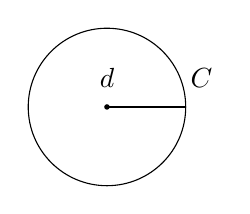
\begin{tikzpicture}

  \draw (0,0) circle [radius=1cm];
  \fill (0,0) circle (1pt);
  \node[label={$d$}] at (0,0) {};
  
  \draw (0,0) -- (1,0); 
  \node[label={$C$}] at (1.2,0) {};
  
\end{tikzpicture}\\

\subsection{Unidade imaginária}
A unidade imaginária $i$ foi criada para resolver equações quadraticas quando a parabola não tocasse o grafico da equação ou seja $b^2 - 4ac<0$.
A unidade imaginária esta sobre um plano complexo que está sobre um plano cartesiano $\mathbb{R}^2$.\\

\begin{tikzpicture}

  \draw (-2,0) -- (2,0);
  \draw(0,-2) -- (0,2);
  
  \fill (2,0) circle (1pt);
  \node[label={$\mathbb{+R}$}] at (2,0) {};
  
  \fill (-2,0) circle(1pt);
  \node[label={$\mathbb{-R}$}] at (-2,0) {};

  \fill (0,-2) circle(1pt);
  \node[label={$-i$}] at (0,-2.7) {};
  
  \fill (0,2) circle(1pt);
  \node[label={$+i$}] at (0,2) {};

\end{tikzpicture}\\

\subsection{Número de Euler}
A primeira descoberta do $e$ foi por Jacob Bernoulli no século XVII quando estudava sobre juros compostos.
Uma conta começa com $\pounds1,00$ e paga juros de $100\%$ ao ano. Se os juros forem creditados uma vez, no final do ano, o valor da conta no final do ano será de $\pounds2,00$.
O que acontecerá se os juros forem calculados e creditados com mais frequência durante o ano?
Se fosse oferecido $50\%$ de juro a cada $6$ meses o valor inicial $\pounds1$ seria $\pounds1.5$, se você esperar mais $6$ meses, você irar receber os $50\%$ do seu restante ou seja $\pounds0.75$
que ficaria com $\pounds2.25$, seria mais ou menos assim $\pounds 1.00 \times 1.5^2 = 2.25$.

\paragraph{Rendimentos trimestrais compostos: $\pounds1.00 \times 1.25^4 = \pounds2.44140625$}
\paragraph{Rendimentos mensais compostos:} $\pounds1.00 \times \left(1+\frac{1}{12} \right)^2 = \pounds2.613035\dots$
\newline
\newline
Leonhard Euler estudou essa propriedade no seu livro \emph{Introdução à análise do infinito} além de provar que o $e$ é um número irracional.

\subsection{Constante Pitagórica}
Para descobrir a Constante Pitagórica usaremos o Teorema de Pitagóras.

\begin{theorem}
O quadrado da hipotenusa é igual a soma dos quadrados dos catetos.
\end{theorem}

traduzindo algebricamente, ficaria assim $\sqrt{a^2+b^2}$.\\

pegue um retangulo $\square$ABCD de comprimento e altura $1$, trace uma reta do ponto B ao ponto C, criando um triangulo reto $\triangle BCD$, use o Teorema de Pitagóras, que ficaria
$\sqrt{1^2+1^2}= \sqrt{2} \approx 1.14$. todo número calculado da um irracional. \\

\centering
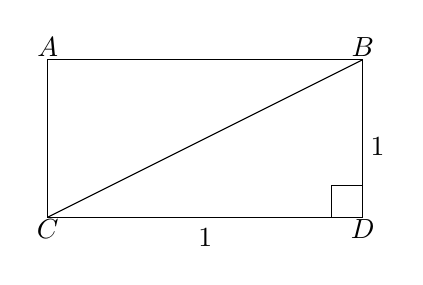
\begin{tikzpicture}

	\draw (0,0) rectangle (4,2);
	\draw (0,2.4) node[anchor=north]{$A$};
	\draw(4,2.4) node[anchor=north]{$B$};
	\draw(0,-0.4) node[anchor=south]{$C$};
	\draw(4,-0.4) node[anchor=south]{$D$};

	\draw(4.4,0.9) node[anchor=east]{$1$};
	\draw(2,-0.5) node[anchor=south]{$1$};
	
	\draw (4,2) -- (0,0); 
	
	\draw (4,0) -- (3.6,0) -- (3.6,0.4) -- (4,0.4) -- cycle;

\end{tikzpicture}



\end{document}
